% !TEX root = ../report.tex
\section{Die Physik}
\begin{Spacing}{\mylinespace}
    Die Physik soll eine möglichst echtzeitfähige und
    realitätsgetreue Simulation von Luftströmung über eine dynamische Landschaft berechnen.
    Zu diesem Zweck sollten die Partikel des Partikelsystem die einzelnen
    Luftteilchen darstellen und mithilfe einer einfachen Physik
    die Interaktion zwischen diesen und ihrer Umgebung simuliert werden.
    \subsection{Komponenten}
        Jedes Luftpartikel besteht aus zwei dreidimensionalen Vektoren.
        Der Vektor $\vec{p}_{i}$ stellt dabei die Position des Partikels im
        Raum dar und der Vektor $\vec{v}_{i}$ beschreibt die aktuelle Bewegung des Partikels.
        Außerdem besitzen alle Partikel den gleichen Radius $r$ und einem
        Reibungskoeffizienten $\mu$, welcher bestimmt wie viel Energie ein Partikel
        bei einer Kollision verliert.
        Zusätzlich zu den Partikeln stehen Informationen über die Umgebung
        wie z.B. Höhendaten der Landschaft und verschiedene externe
        Kräfte ($F$), wie z.B. Gravitation, zur Verfügung.

        %\[ P_{i} = ( \vec{p}_{i}, \vec{v}_{i} ) , P_{i} \in P \]
        %\[ \vec{p}_{i} \in \mathbb{R}^{3} \]
        %\[ \vec{v}_{i} \in \mathbb{R}^{3} \]

        %\[ h_{xy} \in \mathbb{R} \]
        %\[ \vec{f}_i \in \mathbb{R}^{3} \]

    \subsection{Bewegung der Partikel}
        Um die Bewegung der Partikel zu simulieren wird in jeder Iteration,
        für jedes einzelne Partikel, der Bewegungsvektor $\vec{v}_{i}(t)$
        auf den Positionsvektor $ \vec{p}_{i}(t) $ aufaddiert.

        \[ \vec{p}_{i}(t+1) = \vec{p}_{i}(t) + \vec{v}_{i}(t) \]

        Auf diese Weise wird der Impuls solange erhalten bis der Bewegungsvektor
        durch Einwirkung äußerer Kräfte verändert wird (Abbildung \ref{fig:BewegungPartikel}).

        \begin{figure}[h!]
			\centering
			\vspace*{30px}
			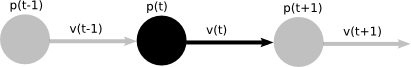
\includegraphics[width=0.7\textwidth]{graphics/Phys_bew0.png}
			\caption{Konstante Bewegung}
			\label{fig:BewegungPartikel}
		\end{figure}

		In diesem Fall wird angenommen das der zeitliche Abstand zwischen den
		einzelnen Iterationen konstant ist. Wenn die Dauer zwischen den Iterationen
		schwankt ist es ratsam dies zu kompensieren indem man den Bewegungsvektor
		$\vec{v}_{i}$ mit dem zeitlichen Abstand ($\Delta t$) zwischen den
		Iterationen multipliziert.
		 \[ \vec{p}_{i}(t+\Delta t) = \vec{p}_{i}(t) + \vec{v}_{i}(t) \cdot \Delta t\]

    \subsection{Verrechnung externer Kräfte}
        In jeder Iteration wird die Wirkung externer Kräfte ($F$) auf das
        Partikel berechnet. Dabei wird jede der externen Kräfte ($\vec{f}_i$) auf den
        Bewegungsvektor $\vec{v}_{i}(t)$ aufaddiert (Abbildung \ref{fig:ModForce}).

        \[ \vec{v}_{i}(t+\Delta t) = \vec{v}_{i}(t) + \sum_{\vec{f}_{i} \in F}{\vec{f}_{i} \cdot \Delta t} \]

		\begin{figure}[h!]
			\centering
			%\subfigure(1){ 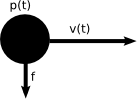
\includegraphics[width=0.2\textwidth]{graphics/Phys_bew1.png} \label{fig:ModForce1} }
			%\subfigure(2){ 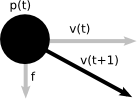
\includegraphics[width=0.2\textwidth]{graphics/Phys_bew2.png} \label{fig:ModForce2} }
			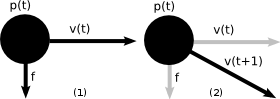
\includegraphics[width=0.4\textwidth]{graphics/Phys_bew12.png}
			\caption{Bewegungsvektor vor(a) und nach(b) Modifikation durch eine externe Kraft }
			\label{fig:ModForce}
		\end{figure}

        Eine externe Kraft ist beispielsweise die Gravitation, welche die Partikel
        in die untere Richtung beschleunigt. Diese Wirkung kann dadurch erzielt
        werden indem beispielsweise der Vektor $( 0,-9.81,0 )$ zu der Menge der externen
        Kräfte hinzufügt wird.
		Diese schrittweise Aufaddierung führt, über mehrere Iteration hinweg gesehen,
		zur Beschleunigung des Partikels, wie es in der Abbildung \ref{fig:bewmod} dargestellt wird.
		\begin{figure}[h!]
			\centering
			\vspace*{30px}
			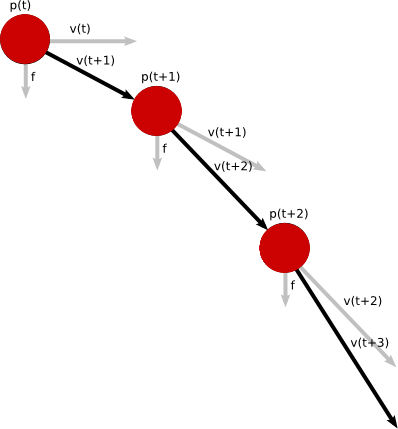
\includegraphics[width=0.7\textwidth]{graphics/Phys_bew3.png}
			\caption{Die auf das Partikel wirkende Kraft(f) bleibt konstant und
			die Bewegung wird bei jedem Rechenschritt weiter in die Richtung der
			Kraft beschleunigt}
			\label{fig:bewmod}
		\end{figure}

    \subsection{Kollisionserkennung von Partikeln mit der Umgebung}
    	Nachdem ein Partikel bewegt wurde, wird überprüft ob eine Kollision mit
    	der Heightmap vorliegt. Eine Kollision liegt vor wenn die vertikale Komponente
    	des Positionsvektors des Partikels einen niedrigeren Wert enthält als der
    	Höhenwert der Heightmap unterhalb der horizontalen Position des Partikels. Wenn dieser Fall
    	vorliegt befindet sich das Partikel unterhalb der Heightmap und ist
    	folglich während der letzten Positionsänderung in das Terrain eingedrungen
    	und es liegt nun eine Kollision vor.

    	Zusätzlich kann der Durchmesser des Partikels berücksichtigt werden
    	indem man den Radius zu dem Höhenwert der Heightmap aufaddiert und
    	dadurch eine Kollision erkannt wird bevor der Positionsvektor unterhalb
    	der tatsächlichen Heightmap liegt.

    \subsection{Kollisionsauflösung von Partikeln mit der Umgebung}
    	Wurde erkannt dass das Partikel mit der Heightmap kollidiert ist, wird eine
    	Kollisionsauflösung durchgeführt. Dabei wird zuerst die Flächennormale
    	der Heightmap ($\vec{n}$) an dem Ort der Kollision berechnet.

    	%\[ \vec{n} = float3((s1 - s3) * coef, 2.0f, (s2 - s4) * coef); \]

    	Mithilfe der Flächennormale $\vec{n}$ wird nun die Reflektion des Bewegungsvektor
    	berechnet und die Bewegungsrichtung auf diese Weise verändert.

    	\[ \vec{v}_{i}(t+1) = \vec{v}_{i}(t+1) -2 \cdot \langle \vec{v}_{i}(t+1) , \vec{n} \rangle \cdot \vec{n} \]

		\begin{figure}[h!]
			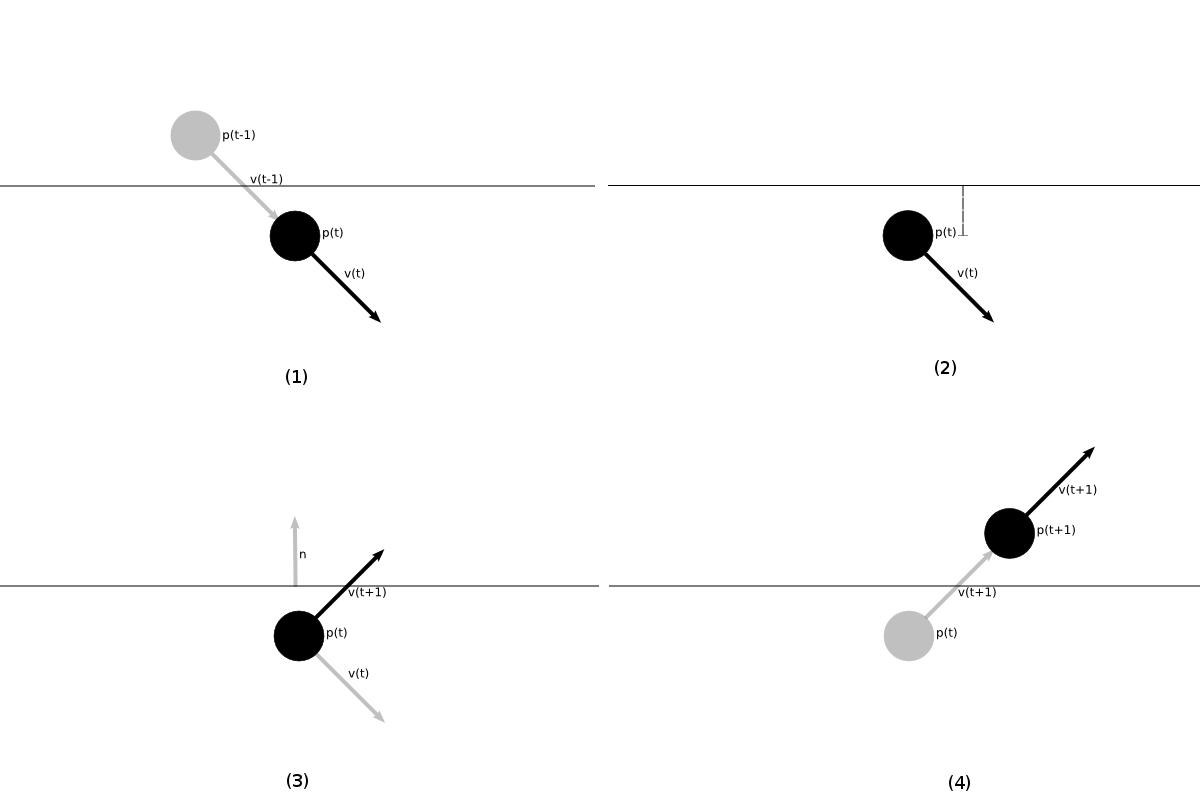
\includegraphics[width=0.99\textwidth]{graphics/Phys_kh1234.png}
			\caption{(a) Partikel dringt in die Heightmap ein. (b) Erkennung der Kollision. (c) Reflektion des Bewegungsvektors(v) entlang der Flächennormale(n). (d) Kollisionsauflösung durch Bewegung in der nächsten Iteration. }
			\label{fig:reflexHeihtmap}
		\end{figure}

		Allein mithilfe der Reflektion können bereits die meisten Kollisionen
		aufgelöst werden. Wenn beispielsweise ein Partikel senkrecht zur Oberfläche
		in die Heightmap eindringt wird der Bewegungsvektor auf diese Weise umgekert
		und das Partikel wird sich in der nächsten Iteration wieder aus der Heightmap
		herausbewegen.
		%\[ \vec{v}_{i}(t) = \left(\begin{array}{rr} 0 \\ 0 \\0 \end{array}\right) , \vec{f}_{i} = \left(\begin{array}{rr} 0 \\ -1 \\0 \end{array}\right) , \vec{n} = \left(\begin{array}{rr} 0 \\ 1 \\0 \end{array}\right) \]
		%\[ \vec{v}_{i}(t+1) = \left(\begin{array}{rr} 0 \\ -1 \\0 \end{array}\right) -2 \cdot \langle \left(\begin{array}{rr} 0 \\ -1 \\0 \end{array}\right) , \left(\begin{array}{rr} 0 \\ 1 \\0 \end{array}\right) \rangle \cdot \left(\begin{array}{rr} 0 \\ 1 \\0 \end{array}\right) = \left(\begin{array}{rr} 0 \\ 1 \\0 \end{array}\right) \]
		\\Die Kombination aus Reflektion und Gravitation führt außerdem dazu, dass
		Partikel die auf der Heightmap liegenbleiben sind, sich entlang des Gefälles
		der Heightmap bewegen, oder im Falle einer horizontalen Ebene auf der aktuellen Position liegenbleiben.
		Dies wird dadurch verursacht, dass ein liegengebliebenes
		Partikel einen Nullvektor als Bewegungsvektor besitzt, wodurch nach Verrechnung der
		Gravitation der Bewegungsvektor dem Vektor der Gravitation entspricht und
		verursacht dass das Partikel in die Heightmap bewegt wird, wodurch eine Kollision hervorgerufen wird.
		Wenn die Flächennormale in die entgegengesetzte Richtung der Gravitation
		zeigt, wie es im Fall einer horizontalen Ebene vorliegt, wird der
		Bewegungsvektor durch die Reflektion vollständig umgekehrt.
		In der nächsten Iteration wird das Partikel wieder an seine
		Ursprungsposition bewegt und die Addition der Gravitation zum Bewegungsvektor führt zur
		Neutralisierung der Bewegung, wodurch der Bewegungsvektor wieder
		zu einem Nullvektor wird und somit die Ausgangssituation wiederhergestellt ist.

		Wenn allerdings die Kollision an einem Gefälle stattfindet, neutralisieren
		sich Bewegung und Gravitation nur teilweise. Da die Gravitation keinen
		Einfluss auf den horizontalen Anteil der Bewegung hat, bleibt dieser
		erhalten und das Partikel bewegt sich in der nächsten Iteration in die
		horizontale Richtung der Flächennormale.
		Auf diese Weise bewegen sich Partikel auf der Oberfläche der Heightmap
		und folgen dabei der horizontalen Richtung der aktuellen Flächennormale.
		Bei einem Gefälle führt dieser Vorgang dazu, dass die Partikel sich,
		wie in Abbildung \ref{fig:rolling} dargestellt ist,
		entlang der schiefen Oberfläche nach unten bewegen, bis sie schließlich
		in einem Tal liegenbleiben. Oder im Fall einer horizontalen Ebene auf der Oberfläche liegenbleiben.
		\begin{figure}[h!]
			\centering
			\vspace*{30px}
			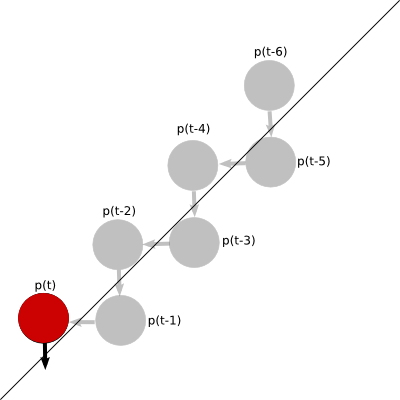
\includegraphics[width=0.7\textwidth]{graphics/Phys_rolling.png}
			\caption{Bewegung eines Partikels entlang eines Gefälles.}
			\label{fig:rolling}
		\end{figure}


		Nach der Reflektion kann die Reibung einbezogen werden, indem der Bewegungsvektor
		$\vec{v}_{i}$ von dem Reibungskoeffizienten $\mu$ gekürzt wird. Wobei $\mu$
		einen festen Wert zwischen 0 und 1 besitzen muss und für alle Partikel gleichermaßen gilt.
		\[ \vec{v}_{i}(t+1) = \vec{v}_{i}(t+1) \cdot ( 1 - \mu ) \]
		Bei dem Wert 1 würde das Partikel alle Bewegungsenergie verlieren und auf der
		Aufprallstelle liegenbleiben. Je kleiner dieser Wert jedoch ist desto weniger
		Energie geht bei einer Kollision verloren und ein Wert von 0 führt dazu, dass
		die Reibung keinen Einfluss mehr auf den Bewegungsvektor hat.

		Die Reibung sorgt dafür, dass die Partikel bei jeder Kollision immer langsamer
		werden, bis sie schließlich vollständig zum erliegen kommen und
		nicht dauerhaft ungebremst und durch die gesamte Welt springen.
		Der Verlust von Bewegungsenergie bedeutet allerdings auch, dass bei einem auf der
		Landschaft liegengebleibenes Partikel die Reflektion nicht mehr vollständig die
		Gravitation ausgleichen kann. Der Bewegungsvektor würde in der
		nächsten Iteration entgegen der Gravitation zeigen, dieser ist allerdings durch die Reibung
		schwächer als die Gravitation und kann diese nun nicht mehr vollständig neutralisieren. Die Reflektion
		reicht nun durch die Kombination mit der Reibung, nicht mehr alleine aus
		um zu verhindern, dass liegengebliebe Partikel immer weiter in die Oberfläche eindringen.

		Um dies zu verhindern wir ein weiterer Mechanismus bei der Kollisionsauflösung benötigt.



    \subsection{Kollisionserkennung zwischen Partikeln} \label{kollpart}
    	Um eine Kollision zwischen zwei Partikeln festzustellen errechnet man
    	den Abstand zwischen beiden indem man beide Positionsvektoren voneinander
    	subtrahiert und den Betrag des daraus resultierenden Vektors ermittelt.
    	Wenn alle Partikel kugelförmig sind,
    	lässt sich eine Kollision sehr einfach ermitteln indem man den Abstand
    	zwischen den Partikeln mit der Summe der beiden Radien der Partikel vergleicht.
    	\[ \vert \vec{p}_{i} - \vec{p}_{j} \vert \leq r_{i} + r_{j} \rightarrow \textrm{Kollision liegt vor} \]
    	\[ \vert \vec{p}_{i} - \vec{p}_{j} \vert > r_{i} + r_{j} \rightarrow \textrm{Keine Kollision} \]
    	Solange der Abstand zwischen beiden Partikeln größer ist als die Summe beider Radien
    	 liegt keine Kollision vor.
    	 \begin{figure}[h!]
			\centering
			\vspace*{30px}
			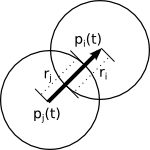
\includegraphics[width=0.2\textwidth]{graphics/Phys_kp.png}
			\caption{Kollisionserkennung durch Vergleich von Abstand und Radien}
			\label{fig:partkoll}
		\end{figure}		
		
		Um alle Kollisionen zu erkennen, müsste in jeder Iteration die Position
		jedes einzelnen Partikels mit den Positionen aller Partikel 
		verglichen werden. Dies führt jedoch dazu, dass in jeder Iteration $n^2$
		Vergleiche durchgeführt werden müssten, was jedoch nur mit einer sehr
		geringen Anzahl an Partikeln praktikabel währe.
		
		Die Gesamtanzahl der Vergleiche lässt sich jedoch dadurch verringern, indem
		die Welt in verschiedene Zellen unterteilt und nur noch
		Kollisionsüberprüfungen zwischen den Partikel innerhalb dieser Kollisionsdomänen
		durchführt werden(Abbildung \ref{fig:partdom}).
		\begin{figure}[h!]
			\centering
			\vspace*{30px}
			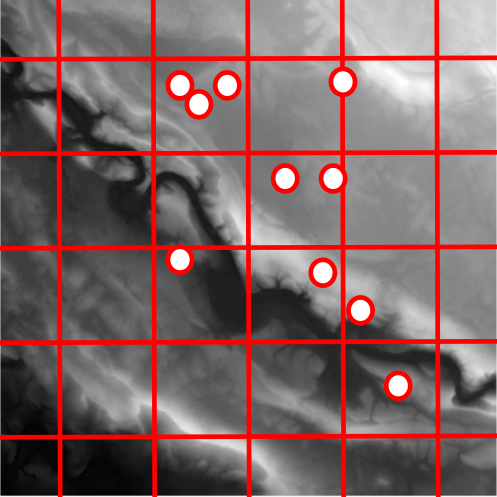
\includegraphics[width=0.6\textwidth]{graphics/Phys_kp_domain.png}
			\caption{Die Aufteilung der Partikel in verschiedene Kollisionsdomänen würde in diesem Beispiel mit 10 Partikeln die Anzahl der Vergleiche von 100 auf nur noch 15 senken.}
			\label{fig:partdom}
		\end{figure}
		
		Die Verteilung der Partikel in Kollisionsdomänen lässt sich mit den
		Möglichkeiten der Shaderprogrammierung unter DirectX9 nicht mithilfe von
		Shadern realisieren und muss daher auf der CPU durchgeführt werden.
		Verursacht wird dieses Problem dadurch, dass es unter DirectX9 nicht
		möglich ist Informationen zwischen den einzelnen Prozessen eines
		laufenden Passes zu teilen.		
		Durch die Notwendigkeit der Neuverteilung der Kollisionsdomänen in jeder
		Iteration, würden jedoch alle Geschwindigkeitsvorteile, die durch die 
		Benutzung der Shader durch die anderen Komponenten entstehen, wieder
		verloren gehen.
		Durch die Umstellung zu Compute Shading liese sich dieses Problem lösen,
		jedoch würde dies zu weitreichenden Veränderungen im gesamten Projekt
		führen.
		
		Wenn die Partikel auf verschiedene Kollisionsdomänen verteilt sind entsteht
		unter DirectX9 ein weiteres Problem. Um die Kollisionen zu erkennen
		werden alle Überprüfungen in einer Schleife durchführt, welche über alle
		beteiligten Partikel iteriert. DirectX9 erlaubt jedoch nur Schiefenstrukturen
		mit einer maximalen Länge von 255 Iterationen, wodurch die
		Köllisionsdomänen so ausgelegt werden müssten dass sich maximal
		255 Partikel in ihnen befinden können.
		
		Die Limitierung der Schleifenlänge ist jedoch nicht die einzige
		Beschränkung die durch DirectX9 und dem Shader Model 3.0 entsteht.
		Dadurch das alle Kontrollstruckturen komplett entfaltet werden, übersteigt die
		die Anzahl der Insruktionen schnell das Instruktionslimit des
		Shader Model 3.0, welches maximal 512 Instruktionen erlaubt.
		Dies reduziert die Anzahl der Kollisionsüberprüfungen
		weiter auf ein unpraktikables Niveau. 
		
		
    \subsection{Kollisionsauflösung zwischen Partikeln}
    	Wenn eine Kollision zwischen Partikeln festgestellt wurde, kann diese in
    	ähnlicher Weise aufgelöst werden wie eine Kollision mit der Heightmap.
    	Um jedoch den Bewegungsvektor des Partikels zu reflektieren, wird die
    	Flächennormale benötigt. Aufgrund der Tatsache dass alle Partikel
    	perfekte Kugeln sind, zeigt die	Flächennormale der Kollisionoberfläche
    	immer in Richtung der Position des Partikels. Daher lässt sich die
    	Flächennormale ($\vec{n}$) dadurch berechnen indem man den Positionsvektor des
    	aktuell betrachteten Partikels ($\vec{p}_{i}$), von dem des mit ihm kollidierenden
    	Partikels ($\vec{p}_{j}$) subtrahiert und dann normiert.
    	\[ \vec{n} = \frac{ \vec{p}_{j} - \vec{p}_{i} }{ \vert \vec{p}_{j} - \vec{p}_{i} \vert } \]
    	\begin{figure}[h!]
			\centering
			\vspace*{30px}
			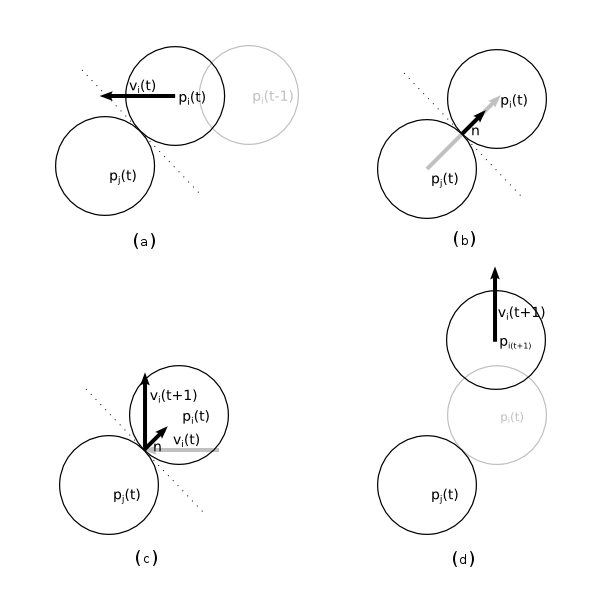
\includegraphics[width=0.7\textwidth]{graphics/Phys_kp1234.png}
			\caption{ (a) Kollision mit einem Partikel. (b) berechnung der Normalen (n). (c) Reflektion des Bewegungsvektors (v). (d) Auflösung der Kollision durch die Bewegung in der nächsten Iteration. }
			\label{fig:partkoll2}
		\end{figure}
		Mit der Flächennormalen ($\vec{n}$) kann nun die Reflektion des
		Bewegungsvektor vorgenommen werden.
		\[ \vec{v}_{i}(t+1) = \vec{v}_{i}(t) -2 \cdot \langle \vec{v}_{i}(t) , \vec{n} \rangle \cdot \vec{n} \]
		Ebenso wie bei der Kollision mit der Heightmap, kann zusätzlich auch
		noch die Reibung und die Flexibilität der Oberfläche einbezogen werden.
	
	\subsection{Flusssimulation}
		Aufgrund der in Kap. \ref{kollpart} genannten Probleme wurde eine
		einfache Flusssimulation implementiert die eine starke Abstraktion
		der Kollision der simmulierten Partikeln mit imaginären Partikel darstellt.
		Diese imaginären Partikel befinden sich zwischen den simmulierten
		Partikeln und der Landschaft, sie werden allerdings weder dargestellt
		noch simmuliert. Dies wird dadurch erreicht indem die Heightmap virtuell
		auf die Höhe des Partikels erhöht, und weder die Wirkung der Gravitation
		noch der Reibung berechnet werden. Erreicht wird dies indem der 
		ewegungsvektor jedes Partikels in jeder Iteration mithilfe der
		Flächennormale der Heightmap unterhalb der Partikelposition
		reflektiert wird.
		Wenn dann Partikel dann in einer horizontalen Bewegung über die 
		Landschaft hinwegfliegen, folgen sie auf diese Weise dem Höhenverlauf
		der Heightmap wie in Abbildung \ref{fig:flow1} dargestellt ist.
		\begin{figure}[h!]
			\centering
			\vspace*{30px}
			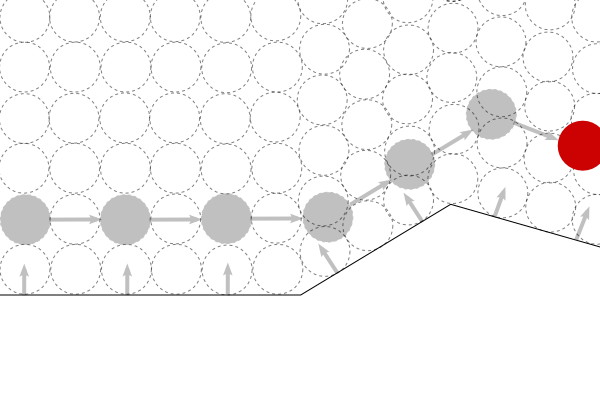
\includegraphics[width=0.7\textwidth]{graphics/Phys_flow1.png}
			\caption{ Bewegung eines Partikels über die imaginären Partikel. }
			\label{fig:flow1}
		\end{figure}
		Diese Technik lässt sich noch weiter verfeinern indem man annimt dass
		die imaginären Partikel je nach Abstand zur Heightmap mehr oder weniger
		beweglich sind. Je näher ein Partikel sich der Heightmap nähert desto
		stärker wird es reflektiert. Befindet es sich jedoch weit über der
		Landschaft verliert die Heightmap den Einfluss auf die Bewegung und der
		Bewegungsvektor wird nicht mehr reflektiert.
		\begin{figure}[h!]
			\centering
			\vspace*{30px}
			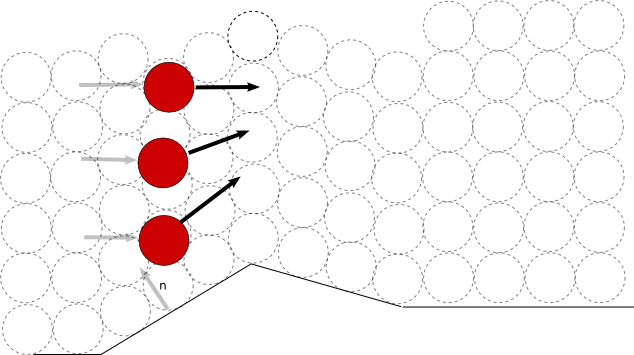
\includegraphics[width=0.7\textwidth]{graphics/Phys_flow2.png}
			\caption{ Manipulation des Bewegungsvektors in verschiedenen Höhen. }
			\label{fig:flow1}
		\end{figure}
		Dies führt mit einfachen Mitteln zu einem bereits ansehnlichen Ergebniss
		welches allerdings nicht wirklich physikalisch korrekt arbeitet.
\end{Spacing}
\newpage
\clearpage
%% End Of Doc
